\documentclass[tikz,border=10pt]{standalone}
\begin{document}
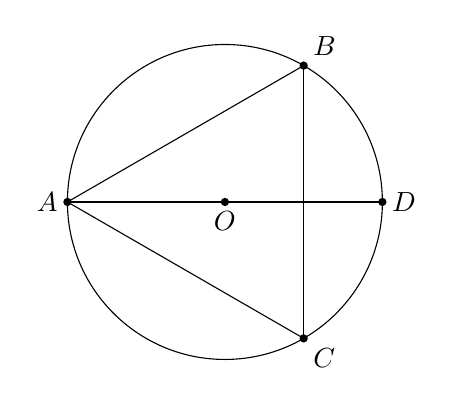
\begin{tikzpicture}
    \coordinate (O) at (0,0);
    \coordinate (A) at (-2,0);
    \coordinate (D) at (2,0);
    \coordinate (B) at (1, {sqrt(3)});
    \coordinate (C) at (1, {-sqrt(3)});

    \draw (O) circle (2);
    \draw (A) -- (D);
    \draw (A) -- (B);
    \draw (A) -- (C);
    \draw (B) -- (C);

    \fill (A) circle (1.5pt);
    \fill (B) circle (1.5pt);
    \fill (C) circle (1.5pt);
    \fill (D) circle (1.5pt);
    \fill (O) circle (1.5pt);

    \node[left] at (A) {$A$};
    \node[above right] at (B) {$B$};
    \node[below right] at (C) {$C$};
    \node[right] at (D) {$D$};
    \node[below] at (O) {$O$};
\end{tikzpicture}
\end{document}
